For the MiniTwit project we have only monitored the backend spring service because it's the heart and the brain to our system. Since the service is hosted in Azure, we have used Azure monitoring features to integrate our service directly with application insight. The configuration requires an AI agent, see “\url{infrastructure-aks/backend/k8s/src/main/resource/AI-Agent.xml}” to be installed and packages within the backend jar file and attached to the service at the class load level. Moreover, we have exposed a set of telemetry to be exposed from spring contest to public. The telemetries we have exposed include health check and information about the service state: up/down, livenessState and readinessState, memory consumption state exposed using the metric probes and service info provided by default in spring-boot-cloud.
\newpage
By integrating with application insight in Azure, we have configured a test health check to send a post request to the health, livenessState and readinessState endpoints exposed from the service and monitor response time the availability state for the service. See Figure \ref{fig:availability} 
\begin{figure}[h]
    \centering
    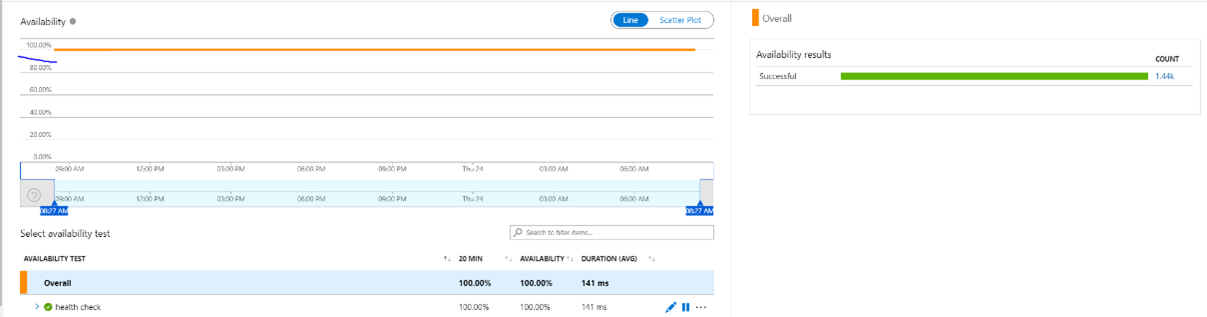
\includegraphics[width = \textwidth]{Availability.png}
    \caption{Screenshot taken of the availability of the system}
    \label{fig:availability}
\end{figure}

Using other previously mentioned exposed metrics, we could see a live capture of system performance, which was during the entire course under 200ms on average. See Figure \ref{fig:metrics} 
\begin{figure}[h]
    \centering
    \begin{subfigure}[b]{0.49\textwidth}
        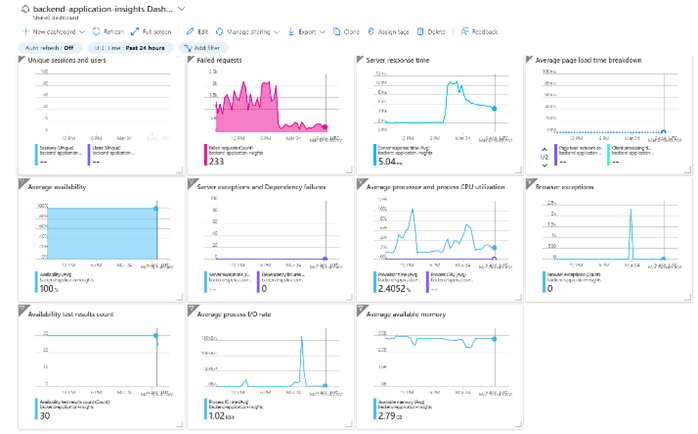
\includegraphics[width =\textwidth]{11things.png}
    \end{subfigure}
    \hfill
        \begin{subfigure}[b]{0.49\textwidth}
        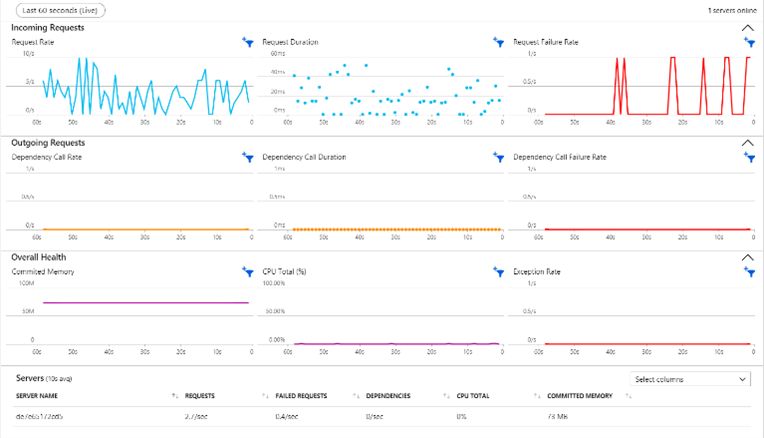
\includegraphics[width =\textwidth]{9things.png}
    \end{subfigure}
    \caption{Metrics exposed in the monitoring process}
    \label{fig:metrics}
\end{figure}

As another alternative for monitoring we used Prometheus and Grafana. They are two powerful monitoring tool used for the visualization of data via charts, graphs, and maps to help us understand behaviors of the system and make decisions. 
 In our project as we are using other monitoring approaches we decided to apply Prometheus and Grafana only on backend, as it's an important part of the system as well as for learning process.
Prometheus can easily be added to a Spring API and combined with Grafana provides visualization.
